\documentclass[11pt]{article}
\usepackage{tikz}

\usetikzlibrary{arrows}

\begin{document}

\section*{FSM for Server}
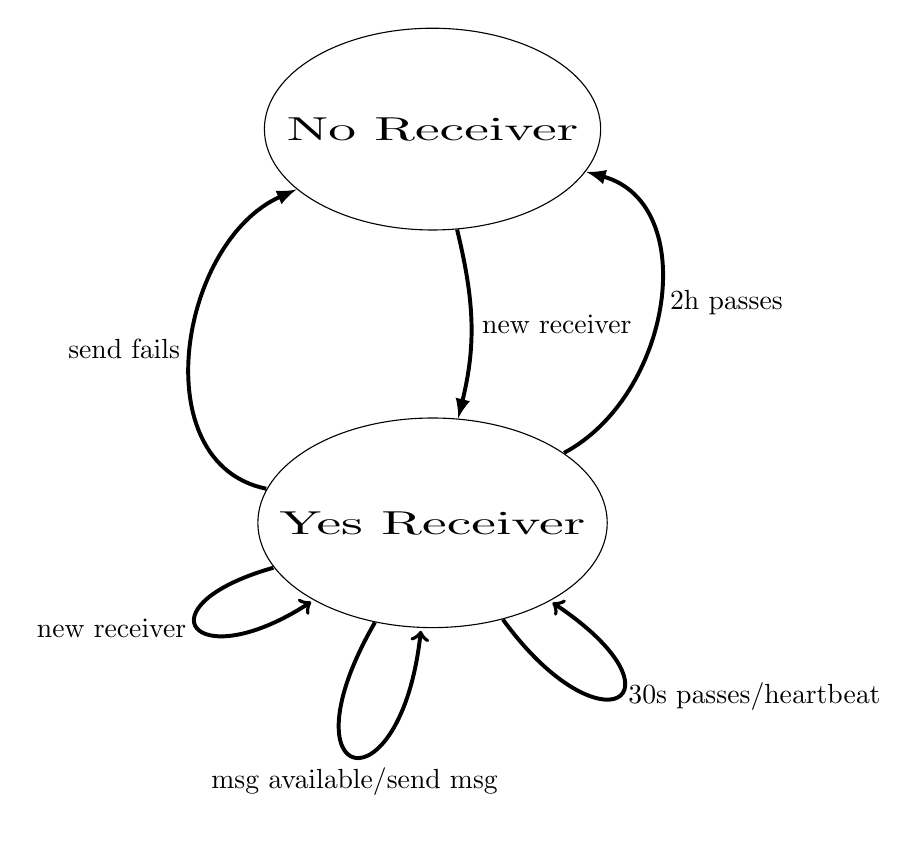
\begin{tikzpicture}
\node[draw, circle, xscale=2, yscale=1.2] at (0,5) (no) {No Receiver};
\node[draw, circle, xscale=2, yscale=1.2] at (0,0) (yes) {Yes Receiver};

%new receiver successfully connects
\draw[arrows={-latex}, line width=.5mm, scale=2]
  (no) to [out=280, in=80] node[right] {new receiver} (yes);
%sending message fails
\draw[arrows={-latex}, line width=.5mm, scale=2]
  (yes) to [out=165, in=210] node[left] {send fails} (no);
%address timeout
\draw[arrows={-latex}, line width=.5mm, scale=2]
  (yes) to [out=35, in=340] node[right] {2h passes} (no);

%self-edges
\path[arrows={-latex}, out=245, in=265, distance=30mm, line width=.5mm]
  (yes) edge[loop] node[below] {msg available/send msg} (yes);
\path[arrows={-latex}, out=300, in=320, distance=30mm, line width=.5mm]
  (yes) edge[loop] node[right] {30s passes/heartbeat} (yes);
\path[arrows={-latex}, out=200, in=220, distance=40mm, line width=.5mm]
  (yes) edge[loop] node[left] {new receiver} (yes);

\end{tikzpicture}

\subsection*{States}
\begin{itemize}
\item No Receiver \\
From the perspective of the Server, the message channel is down, i.e. there is
  no Receiver connected
\item Yes Receiver \\
The message channel is up. The Receiver has connected to the Server recently
and messages should be sent. The Server remains in this state even if the
message channel goes stale.
\end{itemize}

\subsection*{Transitions}
\begin{itemize}
\item No $\rightarrow$ Yes, ``new receiver`` \\
A Receiver successfully connects to the server; the message channel is
established.
\item Yes $\rightarrow$ No, ``send fails'' \\
A message is sent across the message channel but results in \textit{ICMP
unreachable} likely because the underlying holepunch closed.
\item Yes $\rightarrow$ No, ``2h passes'' \\
The \textit{Address timeout} is exceeded. The Server assumes a Receiver will
stay connected to a particular NAT for at most two hours.
\item Yes $\rightarrow$ Yes, ``new receiver'' \\
The Receiver successfully connects from behind a different NAT. The previous
message channel is replaced for the new one.
\item Yes $\rightarrow$ Yes, ``msg available/send msg'' \\
A Sender sends a message to the Server. This message is sent via the message
channel to the Receiver.
\item Yes $\rightarrow$ Yes, ``30s passes/heartbeat'' \\
The Server received no messages within a thirty second window. A heartbeat
message is sent over the message channel to the Receiver to keep the holepunch
open.
\end{itemize}

\pagebreak

\section*{FSM for Receiver}
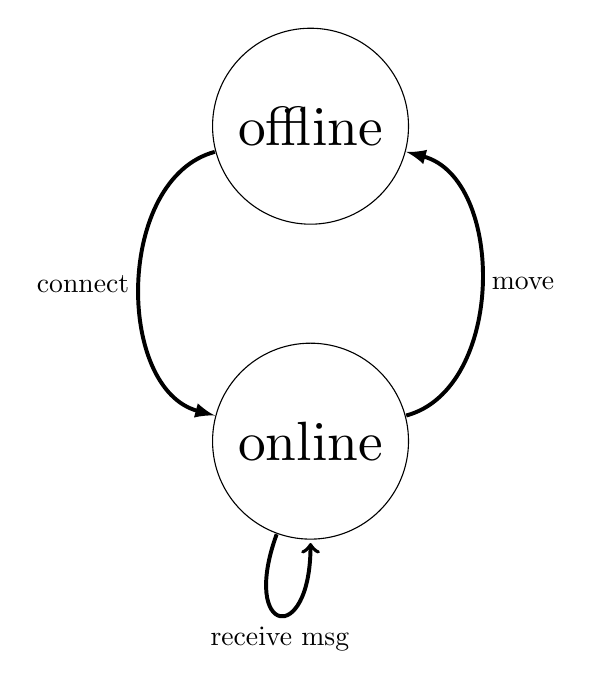
\begin{tikzpicture}
\node[draw, circle, scale=2] at (0,4) (off) {offline};
\node[draw, circle, scale=2] at (0,0) (on) {online};
\draw[arrows={-latex}, line width=.5mm, scale=2] (off) to [out=195, in=165]
  node[left] {connect} (on);
%self edge
\path[arrows={-latex}, out=250, in=270, distance=30mm, line width=.5mm]
  (on) edge[loop] node[below] {receive msg} (on);
\draw[arrows={-latex}, line width=.5mm, scale=2] (on) to [out=15, in=-15]
  node[right] {move} (off);
\end{tikzpicture}

\subsection*{Transitions}
\begin{itemize}
\item offline $\rightarrow$ online ``connect'' \\
The Receiver makes an initial connection to Server, opening a fresh message
channel.
\item online $\rightarrow$ online ``receive msg'' \\
The Server sends a message, either a heartbeat or forwarded from a Sender, via
the message channel to the Receiver.
\item online $\rightarrow$ offline ``move'' \\
The Receiver moves, connecting to a different network or otherwise not
listening on the message channel. This transition is not communicated to the
Server: this is key in the correctness of the protocol.
\end{itemize}
\end{document}
